\section{Casos de Uso}

\begin{figure}[H]
  \begin{center}
  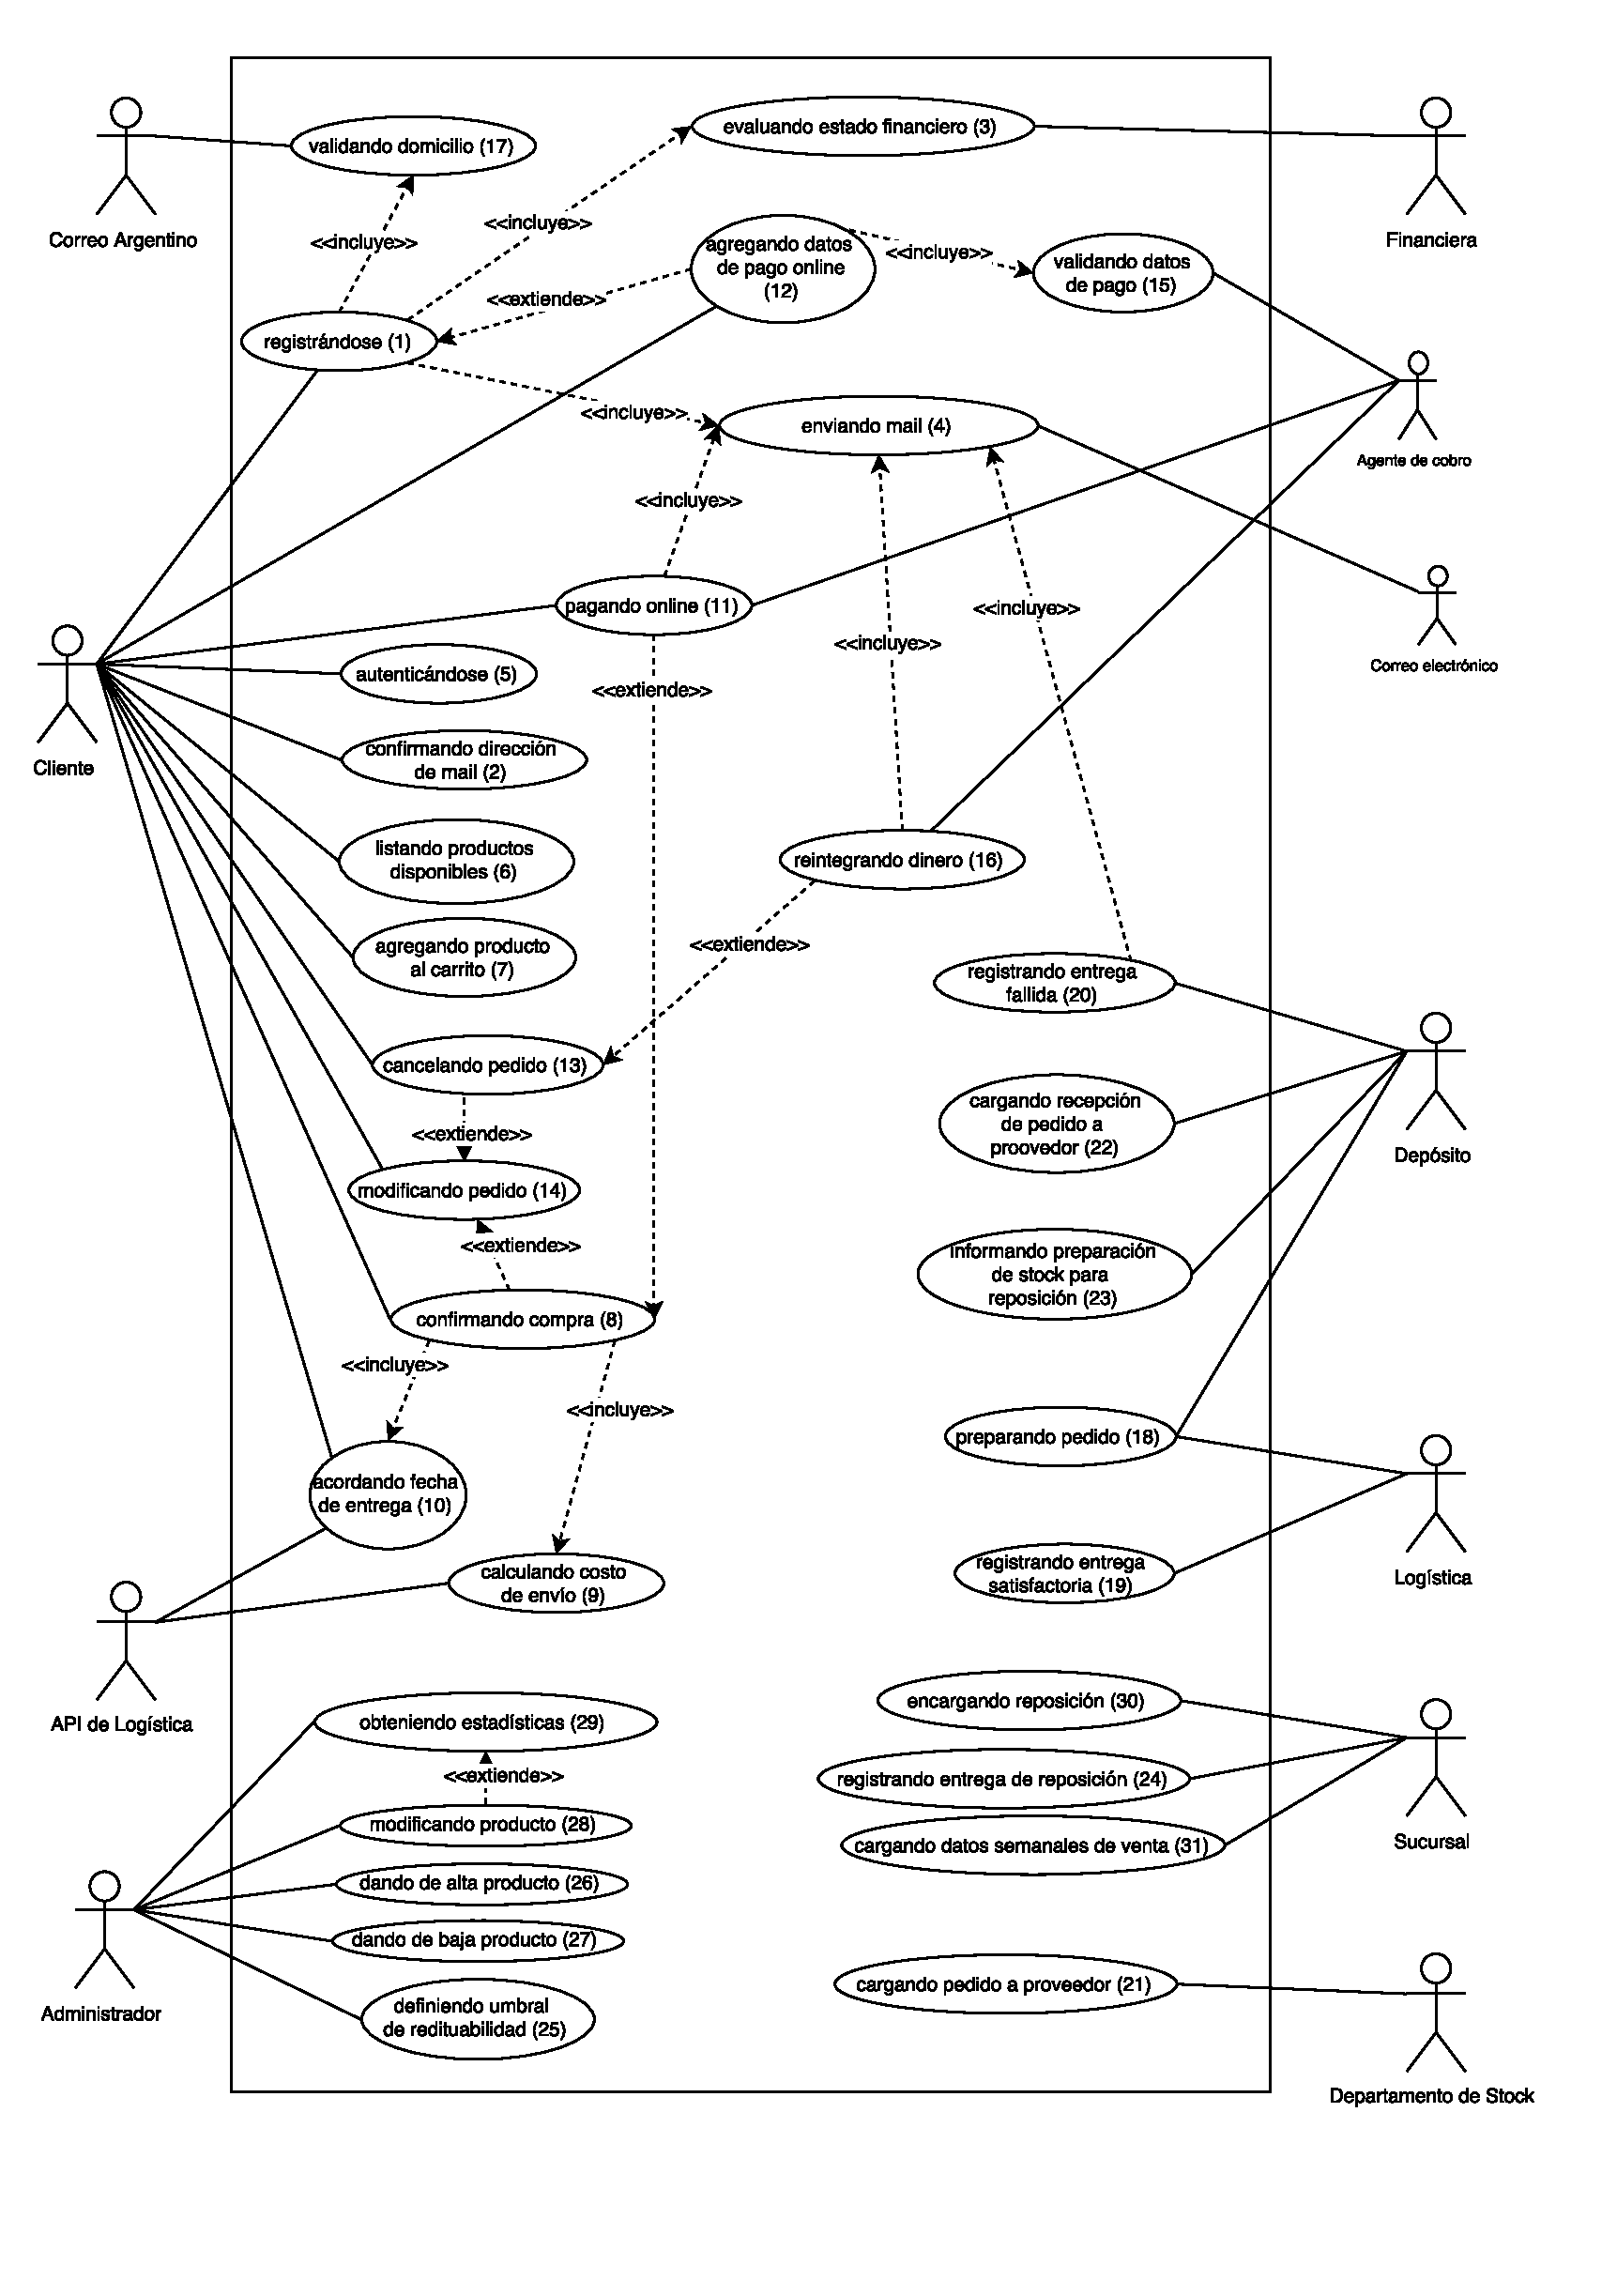
\includegraphics[width=500px]{tp2/images/casos-de-uso.pdf}
  \end{center}
\end{figure}

\captionsetup[table]{name=Caso de uso}


%
% - CASO DE USO: 1) REGISTRANDOSE
%
\begin{casodeuso}
  \cutitle{Registrándose}
  \cuactors{Cliente}
  \cupre{-}
  \cupost{Se ha enviado un mail de bienvenida, el usuario se encuentra pendiente de confirmar.}
  \cucourse{
    1. El cliente ingresa su usuario y contraseña & \\
    2. El sistema valida que el usuario no exista. & 2.1 Si el usuario ya existe, mostrar mensaje e ir a 1. \\
    3. El sistema valida que la contraseña sea segura. & 3.1 Si la contraseña no es segura, informar al cliente e ir a 1 \\
    4. El cliente ingresa sus datos personales & \\
    5. Incluye CU \ref{cu:evaluado-estado-financiero}: evaluando estado financiero & 5.1 Si el cliente tiene deudas, denegarle el registro. FIN CU. \\
    6. El cliente ingresa su dirección & \\
    7. Incluye CU \ref{cu:validando-domicilio}: validando domicilio & 7.1 si el domicilio no es válido, mostrar mensaje de error e ir a 6. \\
    8. Si el cliente desea: es extendido por CU: Agregando datos de pago online & \\
    9. El cliente ingresa su mail & \\
    10. El sistema define el link y el contenido del mail de bienvenida & \\
    11. Incluye CU \ref{cu:enviando-mail}: enviando mail & \\
    12. FIN CU & \\
  }
  \culabel{registrandose}
\end{casodeuso}

%
% - CASO DE USO: 2) CONFIRMANDO DIRECCION DE MAIL
%
\begin{casodeuso}
  \cutitle{Confirmando dirección de mail}
  \cuactors{Cliente}
  \cupre{Se ha enviado un mail de confirmación}
  \cupost{El usuario se confirma}
  \cucourse{
    1. El cliente ingresa al link de confirmación & \\
    2. El sistema marca al usuario como validado & 2.1 Si el link no es válido, se le informa al usuario. \\
    3. FIN CU & FIN CU\\
  }
  \culabel{confirmando-direccion-de-mail}
\end{casodeuso}

%
% - CASO DE USO: 3) EVALUANDO ESTADO FINANCIERO
%
\begin{casodeuso}
  \cutitle{Evaluando estado financiero}
  \cuactors{Financiera}
  \cupre{}
  \cupost{}
  \cucourse{
    1. El sistema envía request a la API de estado financiero con el DNI del cliente & \\
    2. El sistema parsea la respuesta de la API & \\
  }
  \culabel{evaluado-estado-financiero}
\end{casodeuso}

%
% - CASO DE USO: 4) ENVIANDO MAIL
%
\begin{casodeuso}
  \cutitle{Enviando mail}
  \cuactors{Correo electrónico}
  \cupre{El sistema definió un mensaje para un cliente}
  \cupost{Se ha delegado el envío de un correo electrónico}
  \cucourse{
    1. El sistema define el asunto, cuerpo y destinatario (cliente) del nuevo mensaje. & \\
    2. El sistema pide al servidor de correo electrónico enviar el mensaje. & \\
    3. El servidor de correo electrónico confirma el encolamiento del mensaje. & \\
  }
  \culabel{enviando-mail}
\end{casodeuso}

%
% - CASO DE USO: 5) AUTENTICANDOSE
%
\begin{casodeuso}
  \cutitle{Autenticándose}
  \cuactors{Cliente}
  \cupre{}
  \cupost{El cliente se encuentra autenticado}
  \cucourse{
    1. El cliente ingresa el usuario y la contraseña & \\
    2. El sistema verifica los datos ingresados por el cliente & \\
    3. El cliente es redirigido al portal de bienvenida & 3.1 Si los datos son inválidos, se muestra un mensaje de error \\
    4. FIN CU & 4.1 FIN CU\\
  }
  \culabel{autenticandose}
\end{casodeuso}

%
% - CASO DE USO: 6) LISTANDO PRODUCTOS DISPONIBLES
%
\begin{casodeuso}
  \cutitle{Listando productos disponibles}
  \cuactors{Cliente}
  \cupre{El cliente está autenticado}
  \cupost{Se le envió al cliente un listado personalizado de productos}
  \cucourse{
    1. El cliente ingresa al listado de productos & \\
    2. El sistema obtiene los productos que están en stock & \\
    3. El sistema obtiene las recomendaciones para el usuario & \\
    4. El sistema muestra los productos y las recomendaciones que están en stock & \\
    5. FIN CU & \\
  }
  \culabel{listando-productos-disponibles}
\end{casodeuso}

%
% - CASO DE USO: 7) AGREGANDO PRODUCTO AL CARRITO
%
\begin{casodeuso}
  \cutitle{Agregando producto al carrito}
  \cuactors{Cliente}
  \cupre{El cliente tiene el listado de productos}
  \cupost{El producto es agregado al carrito}
  \cucourse{
    1. El cliente hace click sobre el producto & \\
    2. El sistema muestra un dropdown con la cantidad de unidades que están disponibles en ese momento & \\
    3. El cliente elige la cantidad & \\
    4. El sistema agrega el producto al carrito y calcula el monto total  & \\
    5. FIN CU & \\
  }
  \culabel{agregado-producto-al-carrito}
\end{casodeuso}

%
% - CASO DE USO: 8) CONFIRMANDO COMPRA
%
\begin{casodeuso}
  \cutitle{Confirmando compra}
  \cuactors{Cliente}
  \cupre{El cliente tiene un carrito armado}
  \cupost{El cliente tiene una compra reservada y confirmada}
  \cucourse{
    1. El sistema ratifica la disponibilidad de stock para cada producto, y los reserva para el cliente; el carrito se encuentra reservado &  1.1 Si algún producto ya no tiene disponibilidad, se resta del carrito y se le informa al usuario; vuelve al paso 1. \\
    2. Incluye CU \ref{cu:calculando-costo-de-envio}: Calculando costo de envío & \\
    3. El sistema informa del costo total de la compra, incluyendo el envío. & \\
    4. Incluye CU \ref{cu:acordando-fecha-de-entrega}: Acordando fecha de entrega & \\
    5. El sistema determina si el cliente tiene autorizado el pago contraentrega, y presenta los métodos de pagos disponibles & \\
    6. El cliente aprueba el costo y las fechas informadas, e indica el método de pago deseado & \\
    7. Si el pago es online: Es extendido por CU \ref{cu:pagando-online}: Pagando online. & 7.1 Si el pago es online: si el pago no puede ser efectuado, vuelve a paso 7. \\
    8. El pedido es confirmado & 8.1 Si el pedido no pudo ser confirmado luego de 10 minutos, los productos son reingresados a stock, y el carrito deja de estar reservado, vuelve a paso 1 \\
    9. FIN CU & \\
  }
  \culabel{confirmando-compra}
\end{casodeuso}

%
% - CASO DE USO: 9) CALCULAR COSTO DE ENVIO
%
\begin{casodeuso}
  \cutitle{Calculando costo de envío}
  \cuactors{API de Logística}
  \cupre{El domicilio fue previamente validado.}
  \cupost{}
  \cucourse{
    1. El sistema le consulta a la API de logística por el costo de envío hacia el domicilio de un cliente & \\
    2. La API le devuelve al sistema el costo de envío asociado a ese domicilio. & \\
    3. FIN CU & \\
  }
  \culabel{calculando-costo-de-envio}
\end{casodeuso}

%
% - CASO DE USO: 10) ACORDANDO FECHA DE ENTREGA
%
\begin{casodeuso}
  \cutitle{Acordando fecha de entrega}
  \cuactors{Cliente, API de Logística}
  \cupre{El cliente tiene un carrito reservado}
  \cupost{El pedido tiene fecha tentativa de entrega}
  \cucourse{
    1. El sistema pregunta próximas fechas libres a la API de logística & \\
    2. El sistema presenta las posibles fechas al cliente & \\
    3. El cliente elige la fecha deseada & \\
    4. FIN CU & \\
  }
  \culabel{acordando-fecha-de-entrega}
\end{casodeuso}

%
% - CASO DE USO: 11) PAGANDO ONLINE
%
\begin{casodeuso}
  \cutitle{Pagando online}
  \cuactors{Cliente, Agente de Cobro}
  \cupre{El cliente eligió el método de pago online}
  \cupost{El pago del cliente fue acreditado}
  \cucourse{
    1. Si el cliente lo desea, es extendido por CU \ref{cu:agregando-datos-de-pago-online}: agregando datos de pago online & \\
    2. El sistema muestra datos de pago asociados al cliente & \\
    3. El cliente indica método y datos de pago & 3.1 Si el cliente no posee datos de pago, ir a paso 1 \\
    4. El sistema abre una ventana del agente de cobro con los datos de la transacción. & \\
    5. El cliente realiza la operación a través del agente de cobro, generando un token comprobante del pago. & 5.1 Si el agente de cobro rechaza el pago, ir al paso 1.\\
    6. El sistema recibe el comprobante de pago, y lo verifica contra el agente de pago. & 6.1 Si el token de pago es inválido, informar al usuario, e ir al paso 1 \\
    7. El sistema prepara un mail para el cliente, adjuntando un comprobante de pago de la operación.
    8. Incluye CU \ref{cu:enviando-mail}: enviando mail & \\
    9. FIN CU & \\
  }
  \culabel{pagando-online}
\end{casodeuso}

%
% - CASO DE USO: 12) AGREGANDO DATOS DE PAGO ONLINE
%
\begin{casodeuso}
  \cutitle{Agregando datos de pago online}
  \cuactors{Cliente}
  \cupre{El cliente está autenticado}
  \cupost{El cliente posee un nuevo dato de pago asociado a su cuenta}
  \cucourse{
    1. El cliente elige el método de pago online de entre las opciones disponibles & \\
    2. Según el método de pago elegido, el cliente ingresa los datos de autenticación solicitados. & \\
    3. Incluye: validando datos de pago & \\
    4. El sistema asocia los datos de pago a la cuenta del cliente & 4.1 Si los datos de pago son inválidos regresa a paso 1. \\
    5. FIN CU & \\
  }
  \culabel{agregando-datos-de-pago-online}
\end{casodeuso}

%
% - CASO DE USO: 13) CANCELANDO PEDIDO
%
\begin{casodeuso}
  \cutitle{Cancelando pedido}
  \cuactors{Cliente}
  \cupre{El cliente tiene un pedido sin armar en depósito.}
  \cupost{El pedido es cancelado.}
  \cucourse{
    1. Si el carrito está confirmado, la reserva de productos se anula, y los mismos se reingresan a stock. & \\
    2. Si el pedido ya fue pagado de forma online, es extendido por CU \ref{cu:reintegrado-dinero}: Reintegrando dinero & \\
    3. El pedido es cancelado. & \\
    4. FIN CU & \\
  }
  \culabel{cancelando-pedido}
\end{casodeuso}

\textbf{Aclaración sobre corrección previa}: el estado de <<carrito confirmado>> es al que ingresa un pedido
cuando un cliente que se encuentra armando el carrito inicia el proceso de confirmación de compra (por ejemplo
presionando un botón de confirmar compra).
Al ingresar a dicho estado, los productos correspondientes al pedido son restados del stock del depósito, 
y reservados al cliente, de forma tal que luego no puedan ocurrir problemas de stock al intentar 
preparar el pedido. Para más información, ver \textbf{Caso de Uso: \ref{cu:confirmando-compra}}.

%
% - CASO DE USO: 14) MODIFICANDO PEDIDO
%
\begin{casodeuso}
  \cutitle{Modificando pedido}
  \cuactors{Cliente}
  \cupre{El cliente tiene un pedido sin armar en depósito.}
  \cupost{El pedido es cancelado, y un nuevo pedido con las modificaciones es creado.}
  \cucourse{
    1. El cliente quita o agrega los productos que desee, siempre y cuando haya disponibilidad de stock. & \\
    2. Si el carrito está sin confirmar, se registra la modificación & \\
    3. Si el carrito fue confirmado, se cancela el pedido anterior: es extendido por CU \ref{cu:cancelando-pedido} Cancelando Pedido. & \\
    4. Si el carrito fue cancelado, se genera un nuevo pedido con los datos modificados. & \\
    5. Si un nuevo pedido fue generado, es extendido por CU \ref{cu:confirmando-compra}: Confirmando compra. & \\
    6. FIN CU & \\
  }
  \culabel{modificando-pedido}
\end{casodeuso}

%
% - CASO DE USO: 15) VALIDANDO DATOS DE PAGO
%
\begin{casodeuso}
  \cutitle{Validando datos de pago}
  \cuactors{Agente de Cobro}
  \cupre{El cliente ingresó los datos de pago}
  \cupost{Los datos de pago fueron validados}
  \cucourse{
    1. El sistema envía los datos de pago del cliente al Agente de Cobro a través de una API.& \\
    2. El Agente de Cobro informa sobre la validez de los datos de pago. & \\
    3. FIN CU & 3.1 Si los datos de pago no son válidos, el sistema los marca como inválidos, FIN CU\\
  }
  \culabel{validando-datos-de-pago}
\end{casodeuso}

%
% - CASO DE USO: 16) REINTEGRANDO DINERO
%
\begin{casodeuso}
  \cutitle{Reintegrando dinero}
  \cuactors{Agente de cobro}
  \cupre{El cliente canceló un pedido}
  \cupost{El dinero correspondiente al pedido fue reintegrado al cliente}
  \cucourse{
    1. El sistema contacta al agente de cobro, solicitando la anulación de las operaciones correspondientes al pago del pedido. & \\
    2. El agente de cobro anula las operaciones de pago solicitadas, y entrega un número de operación y un comprobante de anulación para cada una de ellas. & \\
    3. El sistema prepara un mensaje para el cliente, informando que el pedido fue anulado, adjuntando los comprobantes de devolución, y lo devuelve al cliente por pantalla. & 3.1 Si el pago no puede ser anulado, se le informa de la situación al cliente, brindándole los números de operación correspondiente.\\
    4. Utilizando el mensaje anterior, incluye caso de uso \ref{cu:enviando-mail}: Enviando mail. & \\
    5. FIN CU & \\
  }
  \culabel{reintegrado-dinero}
\end{casodeuso}

%
% - CASO DE USO: 17) VALIDANDO DOMICILIO
%
\begin{casodeuso}
  \cutitle{Validando domicilio}
  \cuactors{API de Correo Argentino}
  \cupre{El cliente ingresó los datos de su domicilio}
  \cupost{Los datos de domicilio del cliente fueron validados}
  \cucourse{
    1. El sistema envía los datos de domicilio del cliente mediante la API del Correo Argentino & \\
    2. La API del Correo Argentino responde con un mensaje informando la validez del domicilio enviado & \\
    3. FIN CU & \\
  }
  \culabel{validando-domicilio}
\end{casodeuso}

%
% - CASO DE USO: 18) MARCANDO PEDIDO A CLIENTE COMO PREPARADO
%
\begin{casodeuso}
  \cutitle{Marcando pedido como preparado}
  \cuactors{Depósito}
  \cupre{El depósito terminó de preparar un pedido}
  \cupost{El pedido es marcado como preparado}
  \cucourse{
    1. Un operario del depósito carga en el sistema que terminó de preparar el pedido & \\
    2. El sistema marca el pedido como preparado & \\
    3. FIN CU & \\
  }  % por fuera del sistema, deposito le avisa a logistica
  \culabel{marcando-pedido-como-preparado}
\end{casodeuso}

%
% - CASO DE USO: 19) REGISTRANDO ENTREGA SATISFACTORIA
%
\begin{casodeuso}
  \cutitle{Registrando entrega satisfactoria}
  \cuactors{Logística}
  \cupre{Se ha realizado una entrega satisfactoria}
  \cupost{La entrega fue registrada en el sistema}
  \cucourse{
    1. Logística registra la entrega al cliente satisfactoria & \\
    2. Si el pago fue contraentrega, logística carga los datos de recepción del dinero & \\
    3. FIN CU & \\
  }
  \culabel{registrando-entrega-satisfactoria}
\end{casodeuso}

%
% - CASO DE USO: 20) REGISTRANDO ENTREGA FALLIDA
%
\begin{casodeuso}
  \cutitle{Registrado entrega fallida}
  \cuactors{Depósito}
  \cupre{La entrega del pedido fue fallida}
  \cupost{El pedido está anulado y los productos aprobados fueron reingresados a stock}
  \cucourse{
    1. La mercadería en buen estado es reingresada a stock & \\
    2. Depósito carga la falta del cliente y el costo generado a la empresa & \\
    3. El pedido es anulado. & \\
    4. El sistema genera un mensaje conteniendo una invitación a rehacer el pedido, y un link hacia una orden de compra con el mismo carrito del pedido anulado & \\
    5. Incluye CU \ref{cu:enviando-mail}: Enviando mail. & \\
    6. FIN CU & \\
  }
  \culabel{registrando-entrega-fallida}
\end{casodeuso}

%
% - CASO DE USO: 21) CARGANDO PEDIDO A PROVEEDOR
%
\begin{casodeuso}
  \cutitle{Cargando pedido a proveedor}
  \cuactors{Departamento de Stock}
  \cupre{Se hizo un pedido a un proveedor}
  \cupost{El pedido está cargado}
  \cucourse{
    1. El Departamento de Stock carga la información del pedido y su comprobante al sistema. & \\
    2. FIN CU & \\
  }
  \culabel{cargando-pedido-a-proveedor}
\end{casodeuso}

%
% - CASO DE USO: 22) CARGANDO RECEPCIÓN DE PEDIDO A PROVEEDOR
%
\begin{casodeuso}
  \cutitle{Cargando recepción de pedido a proveedor}
  \cuactors{Depósito}
  \cupre{Llegó un pedido al depósito}
  \cupost{Los nuevos productos son ingresados a stock}
  \cucourse{
    1. Depósito registra el ingreso. & \\
    2. El sistema actualiza el stock de los nuevos productos & \\
    3. FIN CU & \\
  }
  \culabel{cargando-recepcion-de-pedido-a-proveedor}
\end{casodeuso}

%
% - CASO DE USO: 23) INFORMANDO PREPARACIÓN DE STOCK PARA REPOSICIÓN
%
\begin{casodeuso}
  \cutitle{Informando preparación de stock para reposición}
  \cuactors{Depósito}
  \cupre{Hay un pedido de reposición de la sucursal}
  \cupost{Los productos requeridos son restados del stock}
  \cucourse{
    1. Depósito informa al sistema que el pedido de reposición se encuentra en preparación. & \\
    2. El sistema resta del stock las unidades correspondientes al pedido. & \\
    3. El sistema le brinda una respuesta al depósito, ofreciendo la descarga de una planilla que contiene un sumario de las unidades que deberán ser enviadas a la sucursal, junto con la información interna que permita agilizar el proceso de preparación (localización dentro del depósito, números de empaque, etcétera). & \\
    4. El  Depósito informa la correcta preparación del pedido. & \\
    5. El sistema marca el pedido preparado, y pone a disposición del Depósito una una hoja de ruta / remito de traslado, para su impresión y futura utilización. & \\
    6. FIN CU & \\
  }
  \culabel{informando-preparacion-de-stock-para-reposicion}
\end{casodeuso}

%
% - CASO DE USO: 24) REGISTRANDO ENTREGA DE REPOSICIÓN
%
\begin{casodeuso}
  \cutitle{Registrando entrega de reposición}
  \cuactors{Sucursal}
  \cupre{Un envío de reposición a sucursal fue entregado correctamente}
  \cupost{La llegada del envío es registrada}
  \cucourse{
  1. La sucursal ingresa al sistema, y marca el pedido de reposición como entregado. & \\
  2. FIN CU. & \\
}
  \culabel{registrando-entrega-de-reposicion}
\end{casodeuso}

%
% - CASO DE USO: 25) DEFINIENDO UMBRAL DE REDITUABILIDAD
%
\begin{casodeuso}
  \cutitle{Definiendo umbral de redituabilidad}
  \cuactors{Administrador}
  \cupre{-}
  \cupost{Se redefine el umbral de redituabilidad}
  \cucourse{
    1. El administrador ingresa el nuevo umbral de redituabilidad & \\
    2. El sistema guarda el nuevo umbral & \\
    3. FIN CU. & \\
  }
  \culabel{definiendo-umbral-de-redituabilidad}
\end{casodeuso}

%
% - CASO DE USO: 26) DANDO DE ALTA PRODUCTO
%
\begin{casodeuso}
  \cutitle{Dando de alta producto}
  \cuactors{Administrador}
  \cupre{-}
  \cupost{El producto solicitado es dado de alta}
  \cucourse{
    1. El administrador ingresa al ABM provisto por el sistema & \\
    2. El administrador ingresa el producto & \\
    3. El sistema da de alta el producto y comunica la operación & \\
    4. FIN CU. & \\
  }
  \culabel{dando-de-alta-producto}
\end{casodeuso}

%
% - CASO DE USO: 27) DANDO DE BAJA PRODUCTO
%
\begin{casodeuso}
  \cutitle{Dando de baja producto}
  \cuactors{Administrador}
  \cupre{-}
  \cupost{El producto solicitado es dado de baja}
  \cucourse{
    1. El administrador ingresa al ABM provisto por el sistema & \\
    2. El administrador ingresa el producto & \\
    3. El sistema da de baja el producto y comunica la operación & \\
    4. FIN CU. & \\
  }
  \culabel{dando-de-baja-producto}
\end{casodeuso}

%
% - CASO DE USO: 28) MODIFICANDO PRODUCTO
%
\begin{casodeuso}
  \cutitle{Modificando producto}
  \cuactors{Administrador}
  \cupre{-}
  \cupost{El producto solicitado es modificado}
  \cucourse{
    1. El administrador ingresa al ABM provisto por el sistema & \\
    2. El administrador ingresa el producto y la modificación & \\
    3. El sistema realiza los cambios solicitados y confirma la operación & \\
    4. FIN CU. & \\
  }
  \culabel{modificando-producto}
\end{casodeuso}

%
% - CASO DE USO: 29) OBTENIENDO ESTADISTICAS
%
\begin{casodeuso}
  \cutitle{Obteniendo estadísticas}
  \cuactors{Administrador}
  \cupre{-}
  \cupost{Se envían las estadísticas al administrador}
  \cucourse{
    1. El administrador solicita las estadísticas a través del sistema & \\
    2. El sistema genera las estadísticas de venta de cada producto y compras de cada usuario, y las prepara para su adecuada visualización & \\
    3. El administrador descarga las estadísticas a través del sistema & \\
    4. Si administrador desea modificar algún producto, es extendido por CU \ref{cu:modificando-producto}: Modificando producto. & \\
    5. FIN CU. & \\
  }
  \culabel{obteniendo-estadisticas}
\end{casodeuso}

Observación: Nos pareció interesante que este caso de uso sea extendido por
la modificación del producto, en particular, del umbral de stock mínimo.
Esta secuencia de eventos está reflejada en el escenario \texttt{L}.

%
% - CASO DE USO: 30) ENCARGANDO REPOSICIÓN
%
\begin{casodeuso}
  \cutitle{Encargando reposición}
  \cuactors{Sucursal}
  \cupre{La sucursal se conecta desde una terminal especial pre-autenticada.}
  \cupost{Los productos deseados fueron encargados}
  \cucourse{
    1. La sucursal ingresa el listado de productos que desea encargar. & \\
    2. El sistema guarda el pedido como pendiente de preparación. & \\
    3. El sistema le confirma a la sucursal que el pedido fue encargado. & \\
    4. FIN CU. & \\
  }
  \culabel{encargado-reposicion}
\end{casodeuso}

%
% - CASO DE USO: 31) CARGANDO DATOS SEMANALES DE VENTA
%
\begin{casodeuso}
  \cutitle{Cargando datos semanales de venta}
  \cuactors{Sucursal}
  \cupre{La sucursal tiene datos de venta para informar}
  \cupost{El sistema contiene datos de venta actualizados}
  \cucourse{
    1. La sucursal carga los datos de venta de la semana a través de una interfaz sencilla, por ejemplo una planilla de cálculos. & \\
    2. El sistema procesa los datos de venta, y los integra a su base de estadísticas & \\
    3. FIN CU. & \\
  }
  \culabel{cargando-datos-semanales-de-venta}
\end{casodeuso}

%
% - CASO DE USO: 32) CONSULTANDO PEDIDO PENDIENTE
%
\begin{casodeuso}
  \cutitle{Consultando pedido pendiente}
  \cuactors{Depósito}
  \cupre{El depósito se conecta desde una terminal especial pre-autenticada.}
  \cupost{El sistema entrega la información del pedido consultado}
  \cucourse{
    1. Un empleado del depósito ingresa al sistema. & \\
    2. El sistema muestra la lista de pedidos pendientes. & \\
    3. El empleado selecciona un pedido y el sistema muestra el detalle. & \\
    4. FIN CU & \\
  }
  \culabel{consultando-pedido-pendiente}
\end{casodeuso}

%
% - CASO DE USO: x) ENVIANDO ALARMA DE BAJO STOCK
%
%\begin{casodeuso}
%\cutitle{21) Enviando alarma de bajo stock}
%\cuactors{Correo electronico}
%\cupre{Existe al menos un producto con stock menor al límite estipulado}
%\cupost{Se avisa de la falta de stock al Departamento de Stock}
%\cucourse{
%1. El sistema prepara una lista de todos los productos por debajo del límite estipulado y el stock necesario para reestablecerlos & \\
%2. El sistema de correo electrónico envía un mail con los datos al Departamento de Stock & \\
%3. FIN CU & \\
%}
%\end{casodeuso}
